\chapter{Testing}

\section{MPU}
The sizes of MPU memory regions are powers of two. This means that the more
memory a partition uses, the more memory it can potentially waste. To combat
this waste, partitions can share MPU memory regions, and be separated
into subregions. This will allow the same level of safety, but more control.
To help optimise the memory layout of partitions a utility program is implemented
that can sort the memory regions of partitions. Each MPU region can contain 8
subregions. All subregions within a region are of equal size.
\\\\
The following is an example of how this utility program can help optimise a
memory layout:
\\

%\begin{figure}[H]
%\centering
%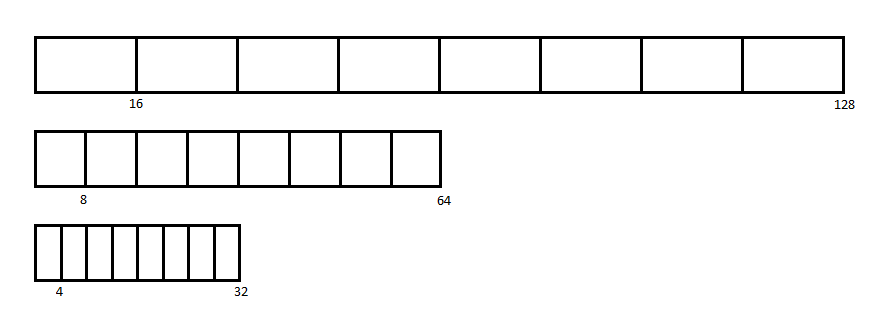
\includegraphics[width=15cm]{partitions/partitions2.png}
%\captionof{figure}{Example of 3 memory region sizes}
%\label{fig:ce1}
%\end{figure}

Assume five partitions with the sizes 20, 65, 120, 80 and 40 bytes, as seen in figure \ref{fig:ce2}.\\

\begin{figure}[H]
\centering
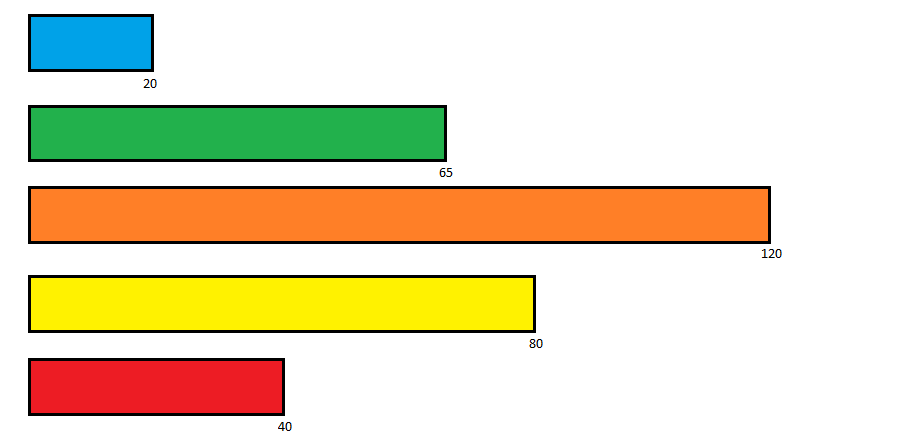
\includegraphics[width=15cm]{partitions/partitions1.png}
\captionof{figure}{An example of 5 partitions of different sizes}
\label{fig:ce2}
\end{figure}

Some of these partitions will waste a lot of memory space if they are allocated their
own memory region. Two of the partitions in particular, the ones with the sizes
65 and 80 bytes, because only they barely cross the 64-byte barrier, needs to be
allocated 128 bytes each.\\
Without optimising the memory layout of the partitions, the memory needed for
all of these would be 480 bytes, which leaves 155 bytes unused. Figure
\ref{fig:ce3} illustrates how each partition would fit in a memory region, and how
much of that memory would be wasted.

\begin{figure}[H]
\centering
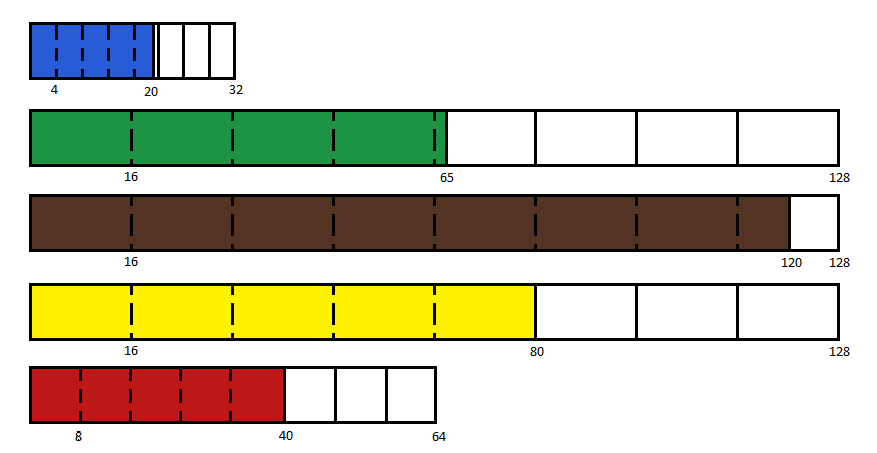
\includegraphics[width=15cm]{partitions/partitions3.png}
\captionof{figure}{An example of a partition memory layout when no partition share a single MPU memory region}
\label{fig:ce3}
\end{figure}

The algorithm for optimising the memory layout is simple. First, allocate a
memory region to the biggest partition. If this partition leaves any unused
subregions, an attempt is made to find the biggest partition fitting into those.
This is continued until all partitions are allocated space.
Once optimised, the five example partitions will only use 384 bytes of memory.
Figure \ref{fig:ce4} shows the optimised memory layout.

\begin{figure}[H]
\centering
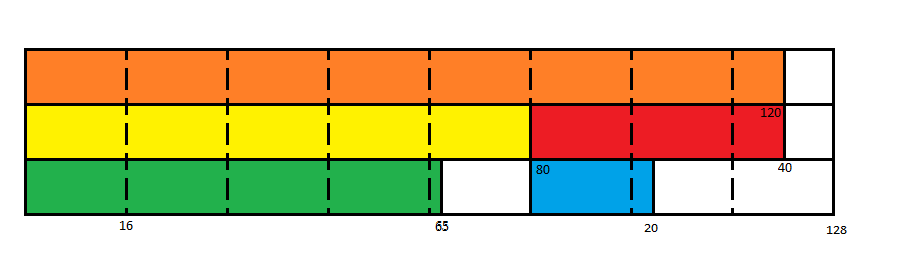
\includegraphics[width=15cm]{partitions/partitions4.png}
\captionof{figure}{An example of an optimised partition memory layout}
\label{fig:ce4}
\end{figure}

Partitions are additionally padded, in case they do not fill an entire the subregion.\\

\begin{figure}[H]
\centering
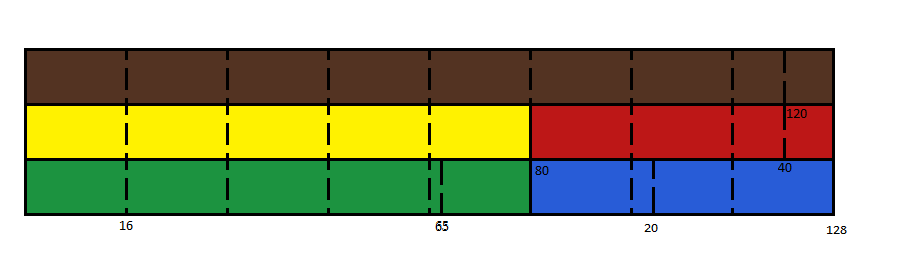
\includegraphics[width=15cm]{partitions/partitions5.png}
\captionof{figure}{An example of how partition memory is padded to fill entire subregions}
\label{fig:ce5}
\end{figure}

%In order to test the memory partition mapping, the sorting memory algorithm is applied and the final
%memory distribution printed in the terminal. For that, the testing environment is setted. Those conditions
%are: the amount of free memory space, the initial memory pointer (to keep track of the start of each
%partition) and each partition size. For the different tests the partition sizes are changed, keeping the
%other 2 unchanged.\\
%Everytime that a partition is allocated, in all its memory positions is written the number of the
%partition. In the the output will be shown the space given to each partition and location in the memory
%map by the number written in each position.\\
%As the sorting algorithm covers different possibilities of partition distributions, according to the
%number of spare subregions (0, 1, 2 or 3), those 4 possibilities were tested, using different
%partition sizes. One of the examples is shown in the image below.\\
%The results printed showed us the subregions distributions and the partition sizes before and
%after the algorithm. The results obtained are exactly like the expected from the mapping algorithm.\\
%
%\begin{figure}[H]
%\centering
%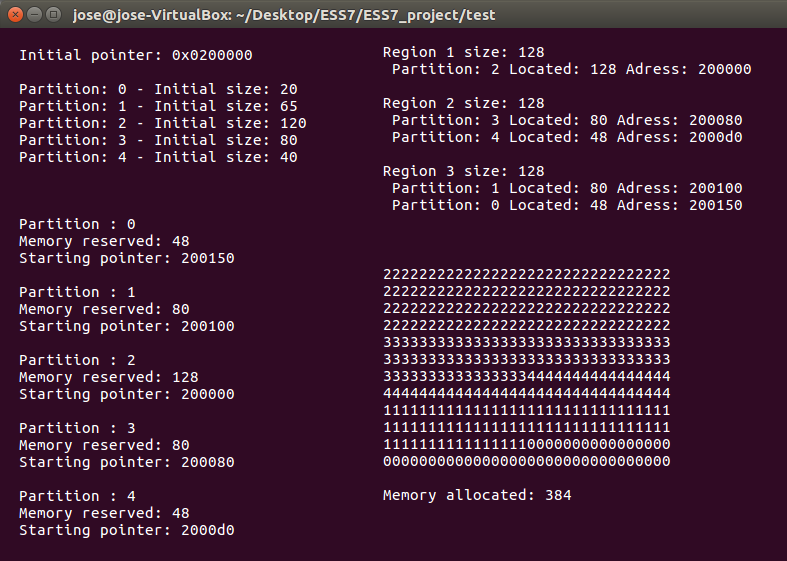
\includegraphics[width=15cm]{mpu_test.png}
%\captionof{figure}{Terminal displaying the results}
%\label{fig:testing_mpu}
%\end{figure}
%
In order to test the memory partition mapping,
the sorting memory algorithm is applied and the final memory distribution printed to the terminal.
The test conditions are:
memory size,
and partition size.
When testing the partition size may change.
The output in figure \ref{ig:testing_mpu} shows the space given to each partition and the location
in the memory map.\\
The results shows the new region sizes containing the larger partitions subregions containing the smaller partitions.
The results corresponds to the mapping the mapping algorithm.

\begin{figure}[H]
	\centering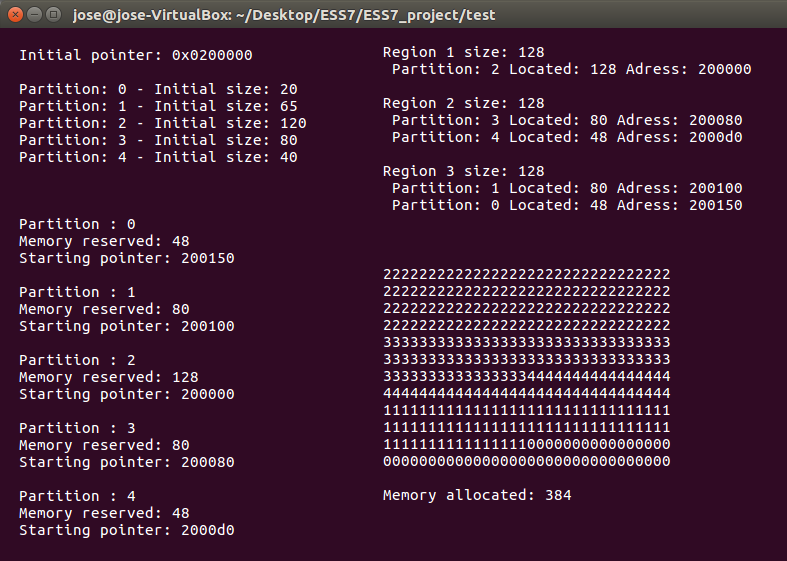
\includegraphics[width=15cm]{mpu_test.png}
	\captionof{figure}{Terminal displaying the results}
	\label{fig:testing_mpu}
\end{figure}


\section{XML validation}
Currently there is no validation of the XML file.
The XML is currently prone to human error when manually
adding to the file, also it does not prevent elements
not compliant with the schema being written.


\section{Scheduler}
The scheduler has been tested to work provided the XML file specifies reasonable
windows. The scheduler has not been tested with edge cases.\\
The kernel does not record any runtime metrics. Empirical
evidence shows that the scheduler is working according to the windows specified in the
XML schema and according to the designed algorithms. Window durations is
scaled up to make it possible with the human eye to determine that the scheduler
indeed follows the windows.


\section{\arinc{} specification - Part 3}
In order to test a system for compliance with \arinc{},
the authors of the standard provide a conformity test
specification. This is a separate document, as a part of the
\arinc{} specification:
\begin{itemize}
	\item\textbf{Part 0} Introduction to ARINC 653
	\item\textbf{Part 1} Required services. This includes system services,
	data structures and functional behaviour.
	\item\textbf{Part 2} Extended services. For example file handling or external events
	\item\textbf{Part 3} \textbf{Conformity test}
	\item\textbf{Part 4} Subset Services
	\item\textbf{Part 5} Core Software Recommended Capabilities
\end{itemize}

Software developers should use this to test the compliance with
Part 1 of the standard. This could be done in the future phases of the \OSname{} OS in order
to demonstrate full compliance of the APEX behavior.


\section{Interpartition Communication}
Interpartition Communication is tested for queuing ports, not sampling ports.
The test is done with the three partitions \texttt{red\_toggler},
\texttt{yellow\_toggler} and \texttt{stdio\_sys}. \texttt{red\_toggler} and
\texttt{yellow\_toggler} broadcast their respective partition name as a string
to the \texttt{stio\_channel}. The \texttt{stdio\_sys} reads any message within its
time-frame and transmits the strings by UART to a connected terminal. Both
transmitting partitions are set to transmit their string every two seconds. A
sample of a recorded output is depicted in figure \ref{fig:message_test},
showing that the communication scheme works as intended.

\begin{figure}[H]
	\centering
	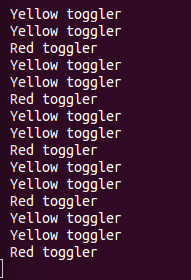
\includegraphics[scale=0.5]{message_test.png}
	\caption{Terminal showing the strings originating from two different
		partitions.}
	\label{fig:message_test}
\end{figure}

As can be seen from the figure, the \texttt{yellow\_toggler} is sending twice as
many messages as \texttt{red\_toggler}. This is due to the scheduling of the two
partitions. The file main\_schema.xml shows that both partitions are
scheduled to execute twice within the major time-frame of 20 seconds, but that
\texttt{yellow\_toggler} is given twice the time of \texttt{red\_toggler} at
every interval and hence gets to print more often.\\

Even though the sampling port module is implemented in the codebase, it is yet
to be fully integrated into \OSname{} and therefore is not tested.
